\documentclass[10pt]{article}

\usepackage[margin=0.75in]{geometry}
\usepackage{amsmath,amsthm,amssymb,bm}
\usepackage{xcolor}
\usepackage{cancel}
\usepackage{graphicx}
\usepackage{changepage}
\usepackage{circuitikz}
\usepackage{pgfplots}
\usepackage{minted}
\usepackage{physics}
\usepackage{hyperref}
\usepackage{siunitx}
\usepackage{fontspec}
\usepackage{relsize}
\usepackage{subfig}
\usepackage{todonotes}
\usepackage{multicol, multirow, booktabs}
\usepackage[breakable]{tcolorbox}
\usepackage[inline]{enumitem}

\theoremstyle{definition}
\newtheorem{problem}{Problem}
\newtheorem{soln}{Solution}

\pgfplotsset{compat=newest}
\usetikzlibrary{lindenmayersystems}
\usetikzlibrary{arrows}
\usetikzlibrary{calc}
\usetikzlibrary{positioning, fit}
\usetikzlibrary{3d, perspective}

\definecolor{incolor}{HTML}{303F9F}
\definecolor{outcolor}{HTML}{D84315}
\definecolor{cellborder}{HTML}{CFCFCF}
\definecolor{cellbackground}{HTML}{F7F7F7}
\newcommand{\ui}{\hat{i}}
\newcommand{\uj}{\hat{j}}
\newcommand{\uk}{\hat{k}}
\newcommand{\ux}{\hat{\mathbf{x}}}
\newcommand{\uy}{\hat{\mathbf{y}}}
\newcommand{\uz}{\hat{\mathbf{z}}}
\newcommand{\uv}[1]{\hat{\bv{{#1}}}}
\newcommand{\pr}[1]{{#1^\prime}}
\newcommand{\pd}[2][]{{\frac{\partial^{#1}}{\partial {{#2}^{#1}}}}}
\newcommand{\dif}[2][]{{\frac{d^{#1}}{d{{#2}^{#1}}}}}
\pgfdeclarelayer{background}  
\pgfsetlayers{background,main}
\AtBeginDocument{\RenewCommandCopy\qty\SI}

\makeatletter
\newcommand{\boxspacing}{\kern\kvtcb@left@rule\kern\kvtcb@boxsep}
\makeatother
\newcommand{\prompt}[4]{
    \ttfamily\llap{{\color{#2}[#3]:\hspace{3pt}#4}}\vspace{-\baselineskip}
}

\newcommand{\thevenin}[2]{
  \begin{center}
    \begin{circuitikz} \draw
      (0,0) -- (2,0) to[battery1, l_=$V_{Th}\eq#1$] (2,2) 
      to[resistor, l_=$R_{Th}\eq#2$] (0,2)
      ;
      \draw [o-] (-.07,2.079);
      \draw [o-] (-.07,0.079);
    \end{circuitikz}
  \end{center}
}

\newcommand{\norton}[2]{
  \begin{center}
    \begin{circuitikz} \draw
      (0,0) -- (3,0) to[american current source, l_=$I_{N}\eq#1$] (3,2) -- (0,2) (2,0)
      to[resistor, l=$R_{N}\eq#2$] (2,2)
      ;
      \draw [o-] (-.07,2.079);
      \draw [o-] (-.07,0.079);
    \end{circuitikz}
  \end{center}
}

\DeclareMathOperator{\Div}{div}
\DeclareMathOperator{\Curl}{curl}
\DeclareMathOperator{\sgn}{sgn}

\newcommand{\highlight}[1]{\colorbox{yellow}{$\displaystyle #1$}}

\newcommand{\ti}[1]{\widetilde{#1}}

\newfontface{\Kaufmann}{Kaufmann}
\DeclareTextFontCommand{\kf}{\Kaufmann}
\newcommand{\scriptr}{\fontsize{12pt}{12pt}\kf{r}}

\newfontface{\KaufmannB}{Kaufmann Bold}
\DeclareTextFontCommand{\kfb}{\KaufmannB}
\newcommand{\bscriptr}{\fontsize{12pt}{12pt}\kfb{r}}
\newcommand{\justif}[2]{&{#1}&\text{#2}}
\newcommand{\bv}[1]{\bm{\mathrm{#1}}}

\title{Physics 3200Y: Assignment VI}
\author{Jeremy Favro (0805980) \\ Trent University, Peterborough, ON, Canada}
\date{\today}

\begin{document}
\maketitle

% PROBLEM 1
\begin{problem}
The space between the plates of a parallel-plate capacitor is filled
with two slabs of linear dielectric. Each slab has thickness $a$, so the total distance between the plates is $2a$.
Slab 1 has a dielectric constant of 2, and slab 2 has a dielectric constant of 1.5. The free charge density on the top plate
is $\sigma$ and on the bottom plate is $-\sigma$.
\begin{enumerate}[label=(\alph*)]
  \item Find the electric displacement $\bv{D}$ in each slab.
  \item Find the electric field $\bv{E}$ in each slab.
  \item Find the polarization $\bv{P}$ in each slab.
  \item Find the potential difference between the plates.
  \item Find the location and amount of all bound charge.
  \item Now that you know all the charge (free and bound), recalculate the filed in each slab, and confirm your answer to (b).
\end{enumerate}
\end{problem}
\begin{soln}~
  \begin{enumerate}[label=(\alph*)]
    \item We have that $$\int \bv{D}\cdot d\bv{a}=Q_{free}=\sigma A$$ and here we expect that
          $\bv{D}$ is entirely in $\uv{z}$ and so the integral jsut becomes $\abs{D}A=\sigma A\implies D=\sigma$.
    \item We also have that $\bv{D}=\epsilon \bv{E}\implies \frac{1}{\epsilon}\bv{D}=\bv{E}$ so we end up with, starting our coordinate system at
          0 and noting that $\epsilon=\epsilon_0\epsilon_r$
          $$
            E=\begin{cases}
              \frac{\sigma}{2\epsilon_0}  & z > a \\
              \frac{2\sigma}{3\epsilon_0} & z < a
            \end{cases}
          $$
    \item We have the $\bv{P}=\epsilon_0\chi_e\bv{E}=\epsilon_0(\epsilon_r-1)\bv{E}$ and hence
          $$
            P=\begin{cases}
              \frac{\sigma}{\epsilon_r\epsilon_0}\epsilon_0(\epsilon_r-1) & z > a \\
              \frac{\sigma}{\epsilon_r\epsilon_0}\epsilon_0(\epsilon_r-1) & z < a
            \end{cases}=
            \begin{cases}
              \frac{\sigma}{2} & z > a \\
              \frac{\sigma}{3} & z < a
            \end{cases}
          $$
    \item This will be the potential due to the field in the first dielectric plus the second dielectric which will turn out as, because the field has no
          position dependence, multiplying the field by $a$, the dielectric thickness. Hence
          $$V=\frac{\sigma a}{2\epsilon_0}+\frac{2\sigma a}{3\epsilon_0}=\frac{7\sigma a}{6\epsilon_0}.$$
    \item Since the polarization has no dependence on position its gradient is zero and hence $\rho_b=-\nabla\cdot \bv{P}=0$. The rest of the bound charge will be at the surfaces
          of the dielectrics and will be given by $\sigma_b=\bv{P}\cdot\uv{n}=\bv{P}\cdot\uz$. At the top of slab 1, nearest the $\sigma$ plate, the bound charge is negative and is
          $-\frac{\sigma}{2}$. At the dielectric interface inside the first dielectric the bound charge is the same but positive so the net charge is conserved. At the interface and inside the
          second dielectric the charge is the negative of what it is at the $-\sigma$ plate, $\frac{\sigma}{3}$ and again so that the net zero charge is conserved the bound charge
          at the bottom plate is $-\frac{\sigma}{3}$
    \item From part (e) we know we have the following charge distribution,
          \begin{center}
            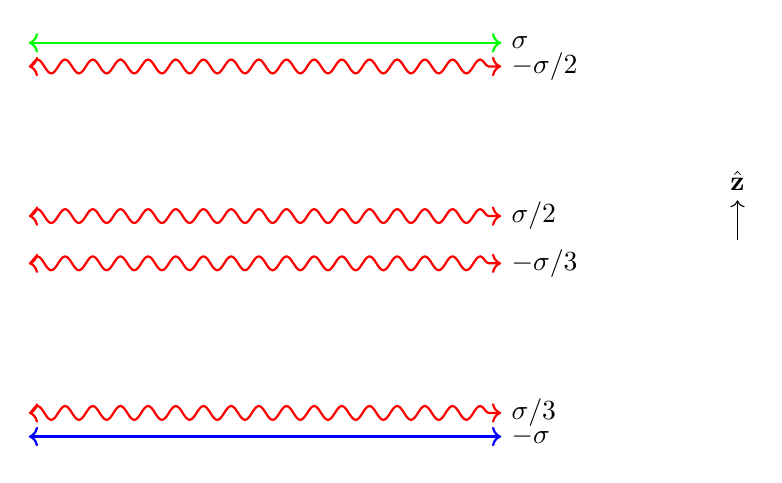
\begin{tikzpicture}
              \tikzset{snake it/.style={decorate, decoration=snake}}

              \def\W{6.0}
              \def\R{2.5}
              \def\S{0.3}

              \draw[<->, green, thick] (0,\R) -- ++(\W,0) node[black, right]{$\sigma$};
              \draw[<->, red, thick, snake it] (0,\R-\S) -- ++(\W,0) node[black, right]{$-\sigma/2$};

              \draw[<->, red, thick, snake it] (0,\S) -- ++(\W,0) node[black, right]{$\sigma/2$};
              \draw[<->, red, thick, snake it] (0,-\S) -- ++(\W,0) node[black, right]{$-\sigma/3$};

              \draw[<->, red, thick, snake it] (0,-\R+\S) -- ++(\W,0) node[black, right]{$\sigma/3$};
              \draw[<->, blue, thick] (0,-\R) -- ++(\W,0) node[black,right]{$-\sigma$};

              \draw[->, black] (\W+3, 0) -- ++(0,0.5) node[above]{$\uz$};
            \end{tikzpicture}
          \end{center}
          which results in an effective charge of $\sigma/2$ at the top plate, $\sigma/6$ in the middle, and $-2\sigma/3$ at the bottom. We know that the electric field due to 
          (one side of) a sheet of charge is given by $$E=\frac{\sigma_P}{2\epsilon_0}$$
          and that electric fields obey linear superposition so we can sum the fields of each plate. These are,
          $$E_{top}=\frac{\sigma}{4\epsilon_0},$$
          $$E_{mid}=\frac{\sigma}{12\epsilon_0},$$
          $$E_{btm}=\frac{\sigma}{3\epsilon_0}.$$
          We do need to be careful about the direction of these fields. The fields due to the top and bottom plates will always point in the $-\uz$ direction when 
          inside the capacitor, and the field due to the middle ``plate'' will point up in the upper region and down in the lower region. Hence the net field in the upper
          region is 
          $$\bv{E}_1=-\frac{\sigma}{4\epsilon_0}\uz+\frac{\sigma}{12\epsilon_0}\uz-\frac{\sigma}{3\epsilon_0}\uz=-\frac{\sigma}{2\epsilon_0}\uz$$
          which is the same as our previous answer. In the lower region,
          $$\bv{E}_2=-\frac{\sigma}{4\epsilon_0}\uz-\frac{\sigma}{12\epsilon_0}\uz-\frac{\sigma}{3\epsilon_0}\uz=-\frac{2\sigma}{3\epsilon_0}\uz$$
          which also corresponds to our previous answer.
  \end{enumerate}
\end{soln}

% PROBLEM 2
\begin{problem}
A very long cylinder of linear dielectric material is placed in an otherwise uniform electric field $\bv{E}_0$. Find the resulting field within the cylinder.
(The radius is $a$, the susceptibility $\chi_e$, and the axis is perpendicular to $\bv{E}_0$.)
\end{problem}
\begin{soln}
  Here we reuse our previously derived solution to $\nabla^2V=0$ in cylindrical coordinates,
  $$V(s,\theta)=A_0+B_0\ln(s)+\sum_{n=1}^{\infty}\left(A_ns^n+B_ns^{-n}\right)\left(C_n\cos(n\theta)+D_n\sin(n\theta)\right).$$
  We are subject to boundary conditions:
  \begin{enumerate}[label=(\roman*)]
    \item $V(s=0)$ is bounded/finite,
    \item $V(s\to\infty)=-E_0s\cos\theta$ where the potential comes from the given electric field,
    \item $V_{O}(s=a)=V_{I}(s=a)$,
    \item $\eval{(\epsilon_0\bv{D}_O-\epsilon \bv{D}_I)}_{s=a}cdot \uv{n}=\eval{(-\epsilon_0\nabla V_O+\epsilon \nabla V_I)}_{s=a}\cdot \uv{n}=0$ as there is no free charge.
  \end{enumerate}
  From boundary condition (i) we see that 
  $$V_I=A_0+\sum_{n=1}^{\infty}\left(A_ns^n\right)\left(C_n\cos(n\theta)+D_n\sin(n\theta)\right).$$
  And from boundary condition (ii) we see that 
  $$V_O=-E_0s\cos\theta=\lim_{s\to\infty}\pr{A}_0+\pr{B}_0\ln(s)+\sum_{n=1}^{\infty}\left(\pr{A}_ns^n+\pr{B}_ns^{-n}\right)\left(\pr{C}_n\cos(n\theta)+\pr{D}_n\sin(n\theta)\right)$$
  which implies that $\pr{A}_0=\pr{B}_0=\pr{D}_n=0\forall n$ and that $\pr{A}_n\pr{C}_n=0\forall n\neq1, \pr{A}_1\pr{C}_1=-E_0$ and hence 
  $$V_O=-E_0s\cos\theta+\sum_{n=1}^{\infty}\pr{B}_ns^{-n}\left(\pr{C}_n\cos(n\theta)+\pr{D}_n\sin(n\theta)\right).$$
  Boundary condition (iii) says that 
  $$
  A_0+\sum_{n=1}^{\infty}\left(A_na^n\right)\left(C_n\cos(n\theta)+D_n\sin(n\theta)\right)
  =
  -E_0a\cos\theta+\sum_{n=1}^{\infty}\pr{B}_na^{-n}\left(\pr{C}_n\cos(n\theta)+\pr{D}_n\sin(n\theta)\right)
  $$
  and so $A_0=0$
  $$
  \sum_{n=1}^{\infty}\left(A_na^n\right)\left(C_n\cos(n\theta)+D_n\sin(n\theta)\right)
  =
  -E_0a\cos\theta+\sum_{n=1}^{\infty}\pr{B}_na^{-n}\left(\pr{C}_n\cos(n\theta)+\pr{D}_n\sin(n\theta)\right)
  $$
  which tells us that $D_n=\pr{D}_n=0\forall n$ and that $A_nC_n=\pr{C}_n\pr{B}_n=0\forall n\neq 1$
  but for $n=1$ these give us that 
  $$A_1C_1a=-E_0a+\pr{C}_1\pr{B}_1a^{-1}.$$
  We'll say that $A_1C_1=F$, $\pr{C}_1\pr{B}_1=G$, so 
 $$ 
    Fa=-E_0a+Ga^{-1}.
    =Ga^{-1}
  $$
  Now boundary condition (iv) says that
    $$
  \epsilon F\cos(\theta)
  =
  -E_0\epsilon_0\cos\theta-\epsilon_0Ga^{-2}\cos(\theta)
  $$
  we can cancel out the $\epsilon_0$ to obtain 
    $$
  (1+\chi_e)F
  =
  -E_0-Ga^{-2}
  $$
  which says that 
      $$
  F
  =-\frac{E_0+Ga^{-2}}{(1+\chi_e)} \implies F=-\frac{E_0}{1+\chi_e/2}
  $$
  which gives us a potential inside of 
  $$V_I=-\frac{E_0}{1+\chi_e/2}s\cos\theta=-\frac{E_0}{1+\chi_e/2}x\implies \bv{E}_{inside}=\frac{E_0}{1+\chi_e/2}\ux$$
\end{soln}

% PROBLEM 3
\begin{problem}
A spherical conductor, of radius $a$, carries charge $Q$.
It is surrounded by linear dielectric material of susceptibility $\chi_e$, out to radius $b$. Find the energy of this configuation.
\end{problem}
\begin{soln} To do this we'll need both the electric field and the electric displacement. To obtain the electric field we just need the displacement so that's all we'll 
get. Inside the conductor the displacement is zero as usual, and for $r>a$ we can use Gauss' law,
$$\int \bv{D}\cdot d\bv{a}=Q\implies \bv{D}=\frac{Q}{4\pi r^2}\uv{r}.$$
The electric field is given by $E=D/\epsilon$ and hence has three values. Inside the conductor it is zero. For $a<r<b$, $$\bv{E}=\frac{Q}{4\pi\epsilon_0(1+\chi_e) r^2}\uv{r}$$
and for $r>b$ it is $$\bv{E}=\frac{Q}{4\pi\epsilon_0 r^2}\uv{r}.$$
We can now use the work integral for a dielectric, 
$$W=\frac{1}{2}\int\bv{D}\cdot\bv{E}\,d^3r=\frac{Q^24\pi}{2(4\pi)^2\epsilon_0}\left[\frac{1}{1+\chi_e}\int_{a}^{b}\frac{1}{r^4}r^2dr+\int_{b}^{\infty}\frac{1}{r^4}r^2dr\right]
=\frac{Q^2}{8\pi\epsilon_0}\left[\frac{1}{1+\chi_e}\left(\frac{1}{a}-\frac{1}{b}\right)+\frac{1}{b}\right]
$$
\end{soln}
\end{document}